%!TEX TS-program = ../make.zsh

\subsection{Unit Tests and Consistency Checks}
\label{sec:unit_tests_and_cross_checks}

\todo{Paragraph about several kinds of tests}

- single photons, unit tests
- several photons behaving the same way, instant absorption
- sample several photons, statistical properties, distribution of observables like arrival time or path length, qualitatively, quantitatively

### Unit Tests With Single Photons
\label{sec:unit_tests}

In order to verify that individual components (``units'') of the implementation perform their tasks as expected, that is to say produce results as expected, unit tests were implemented for the algorithm that calculates intersections as well as for the hole-ice-correction algorithm.

\sourcepar{The unit tests for the intersection algorithm can be found at \url{https://github.com/fiedl/clsim/blob/sf/hole-ice-2017/resources/kernels/lib/intersection/intersection_test.c}, the unit tests for the hole-ice-correction algorithm at \url{https://github.com/fiedl/clsim/blob/sf/hole-ice-2017/resources/kernels/lib/hole_ice/hole_ice_test.c}.}

\paragraph{Task} The task of unit tests is to test individual components of a software. In this case, the tests execute separate functions of the new algorithms with fixed input parameters and check whether the functions return the expected results that, in preparation of the test, have been obtained by other means, either by a separete program, using a separate programming language, a separate algorithm, or via calculations by hand.

In this study, unit tests implement single photons that cross hole-ice cylinders in a pre-defined way and check whether the intersection algorithm determines the correct intersection points, whether the 2d-3d projections are handled correctly, and whether the hole-ice-correction algorithm determines the expected corrections for the geometric distances according to the hole-ice parameters provided by the test scenario.

Extreme examples can be designed to produce simple results that can be calculated by hand and verified by intuition. For example, for hole-ice cylinders configured for instant absorption, the absorption point is identical to the intersection point of the photon trajectory and the cylinder.

More complex examples require more involved calculations by hand or using other software like \noun{Python} scripts or specialized tools like \noun{GeoGebra}\footnote{GeoGebra mathematical tools, \url{https://www.geogebra.org}} (see figure \ref{fig:Uchie2aa}) for calculating intersections.
% https://github.com/fiedl/hole-ice-study/issues/20
% https://github.com/fiedl/hole-ice-study/issues/25

% \begin{figure}[htbp]
%   \image{geogebra}
%   \caption{A specialized software tool like \noun{GeoGebra} can be used to obtain or verify individial calculation results, which then are used in unit tests to verify the results of the implemented algorithms.}
%   \label{fig:Uchie2aa}
% \end{figure}

\paragraph{Testing Framework}
This study uses the \noun{gtest}\footnote{Google Test Framework, gtest, \url{https://github.com/google/googletest}} testing framework.

% Notes: 2017-07-21
This framework has been chosen due to its good documentation, wide adoption and slim architecture that made it possible to use the framework to test individual components of the new source code without interfering with the rest of the icesim framwork.

\docpar{The introductory documentation of gtest can be found at \url{https://github.com/google/googletest/blob/master/googletest/docs/primer.md}.}

\paragraph{Pros and Cons}
Unit tests are most useful to ensure stability when adjusting, refactoring or rewriting software components. Even after replacing a large source code, unit tests can make sure that the software still produces the same results as before.

Tests also allow for so-called test-driven development where the expected results are specified first, and then the software is built or changed iteratively until it produces the expected results.

This technique works best when the components to be tested have small interfaces because the technique requires the tests to provide all input paramters for the components to be tested.

Unexpected issues may arise when unit tests are run on another architecture as the production code. For example, the unit tests used in this study were insensitive to certain driver issues and numerical issues\footnote{\mref{technical-issues section}} that did only occur when running the software on the GPUs of the computing cluster and did not occur when running the unit tests on the local CPU of the development machine.

Unit tests are, by design, also insensitive to high-level problems. Each individual component may produce the results expected from this component while still issues may arise when components are not tied together correctly, or because the expectations for an individual component may be wrong, which becomes apparent only when adopting a larger perspective rather than the focused perspective on individual components.

To increase confidence in the new software, therefore, in addition to unit testing, high-level consistency checks need to be performed as described in the following subsections.


### Instant-Absorption Tests

A simple high-level test can be performed by starting photons towards a cylinder, which is configured for instant absorption. After propagating the photons using the new media-propagation algorithm and recording the path of each individual photon, one can verify the results using a python script that makes sure than no recorded photon position is inside the instant-absorption cylinder.

Additionaly, one can visualize the simulation using the \noun{Steamshovel} event viewer to verify that no photon enters the instant-absorption cylinder as shown in figure \ref{fig:moo9Eiqu}.

% instant absorption: issue #22

\begin{figure}[htbp]
  \begin{subfigure}{.5\linewidth}
    \image{instant-absorption-steamshovel-moo9Eiqu}
    \caption{Starting from different positions into the same direction. View from above.}
  \end{subfigure}
  \begin{subfigure}{.5\linewidth}
    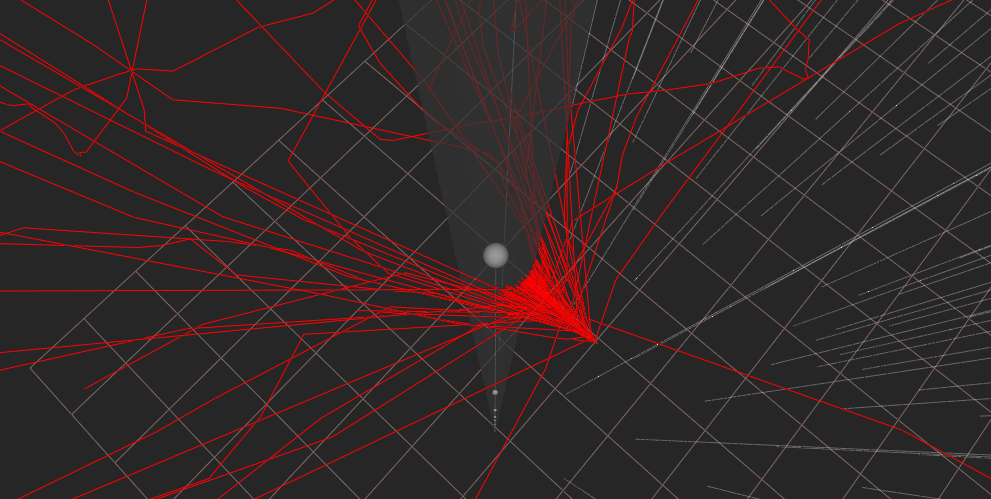
\includegraphics[width=\textwidth, trim={0 0 40mm 0}, clip]{img/instant-absorption-steamshovel-Zae4phei}
    \caption{Starting from the same position into different directions.}
  \end{subfigure}
  \caption{Visualizing an instant-absorption test using the \noun{Steamshovel} event viewer. In the simulation, photons are started towards a cylinder configured for instant absorption. If the medium-propagation algorithm works as expected, no photon can get inside the cylinder.}
  \label{fig:moo9Eiqu}
\end{figure}

A related, but more complex scenario is starting photons within two nested cylinders where the inner cylinder is configured for a short scattering length and the outer cylinder is configured for instant absorption (figure \ref{fig:sahmoo8O}).

% https://github.com/fiedl/hole-ice-study/issues/47

\begin{figure}[htbp]
  \begin{subfigure}{.32\linewidth}
    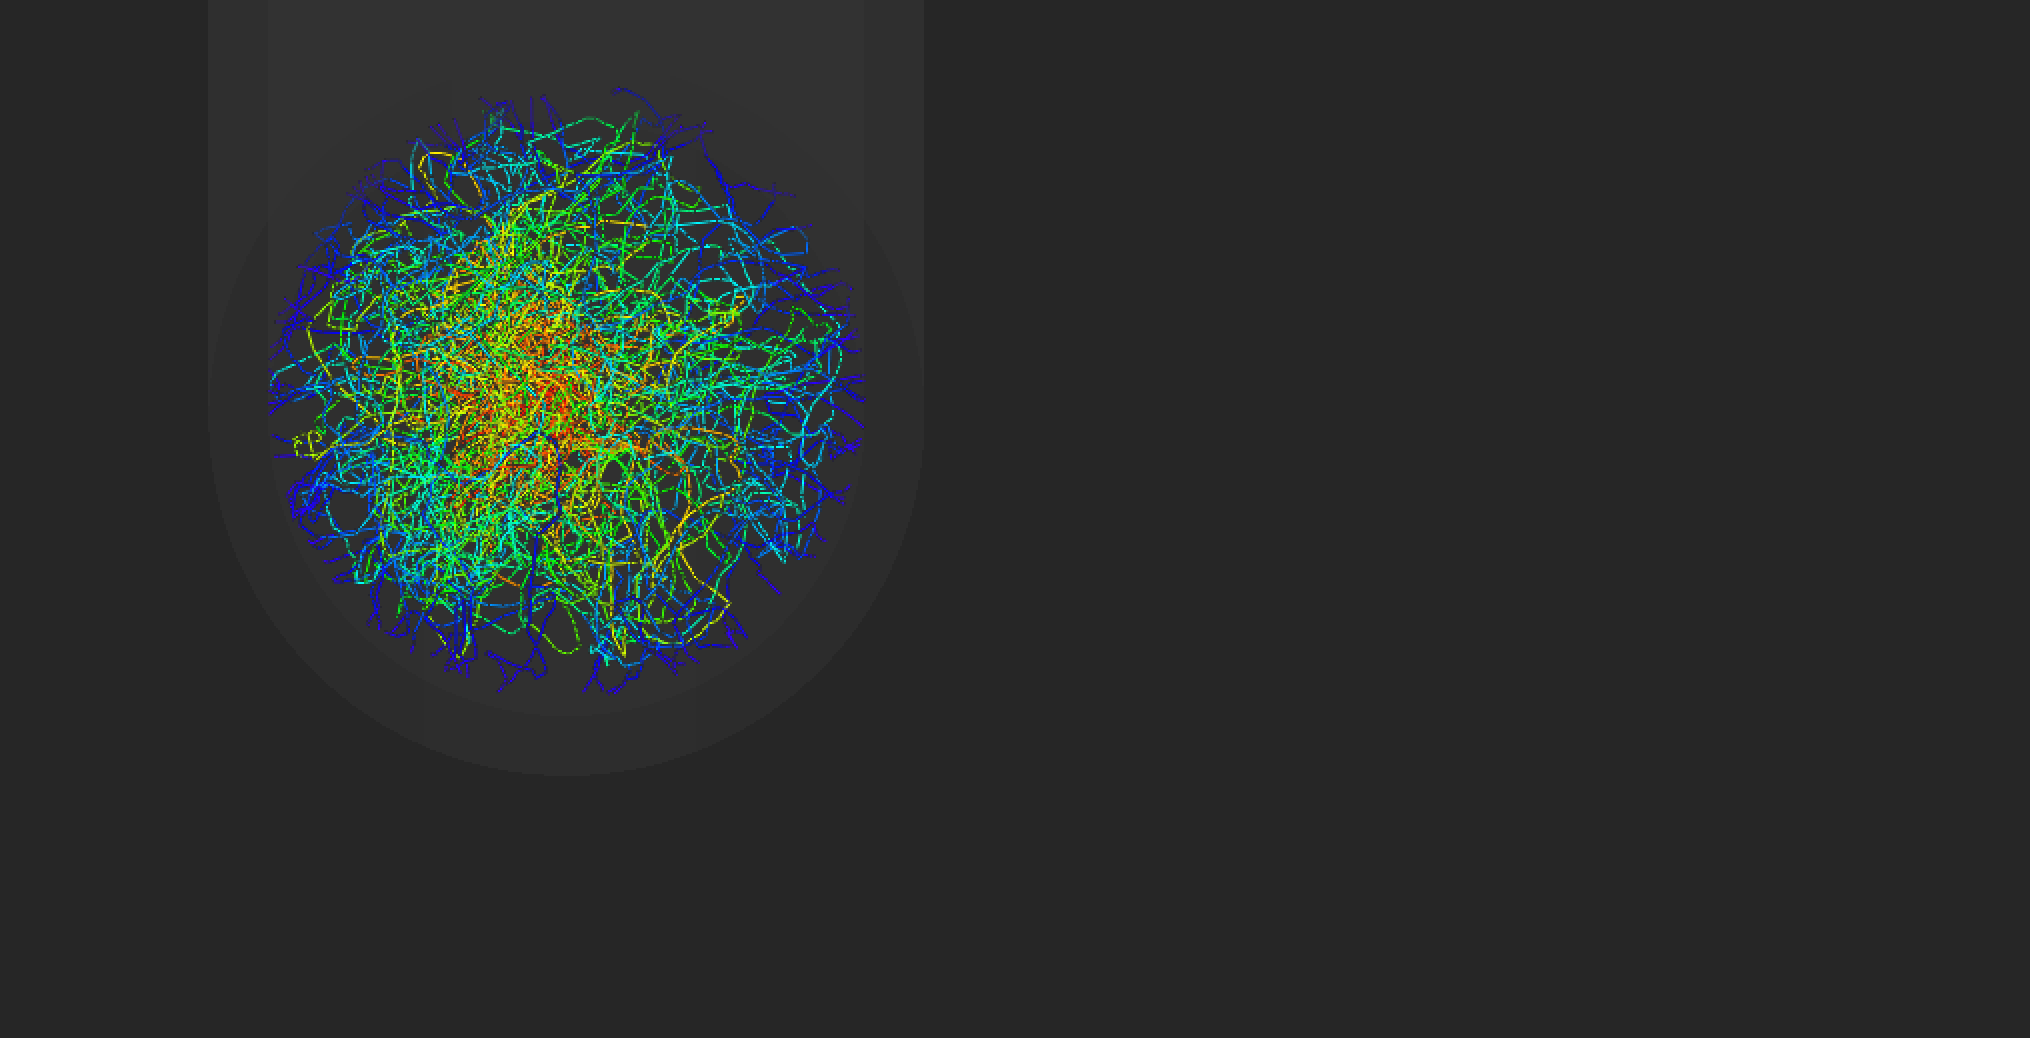
\includegraphics[width=\textwidth, trim={0 3cm 16cm 0}, clip]{img/instant-absorption-steamshovel-sahmoo8O-above}
    \caption{View from above.}
  \end{subfigure}
  \begin{subfigure}{.32\linewidth}
    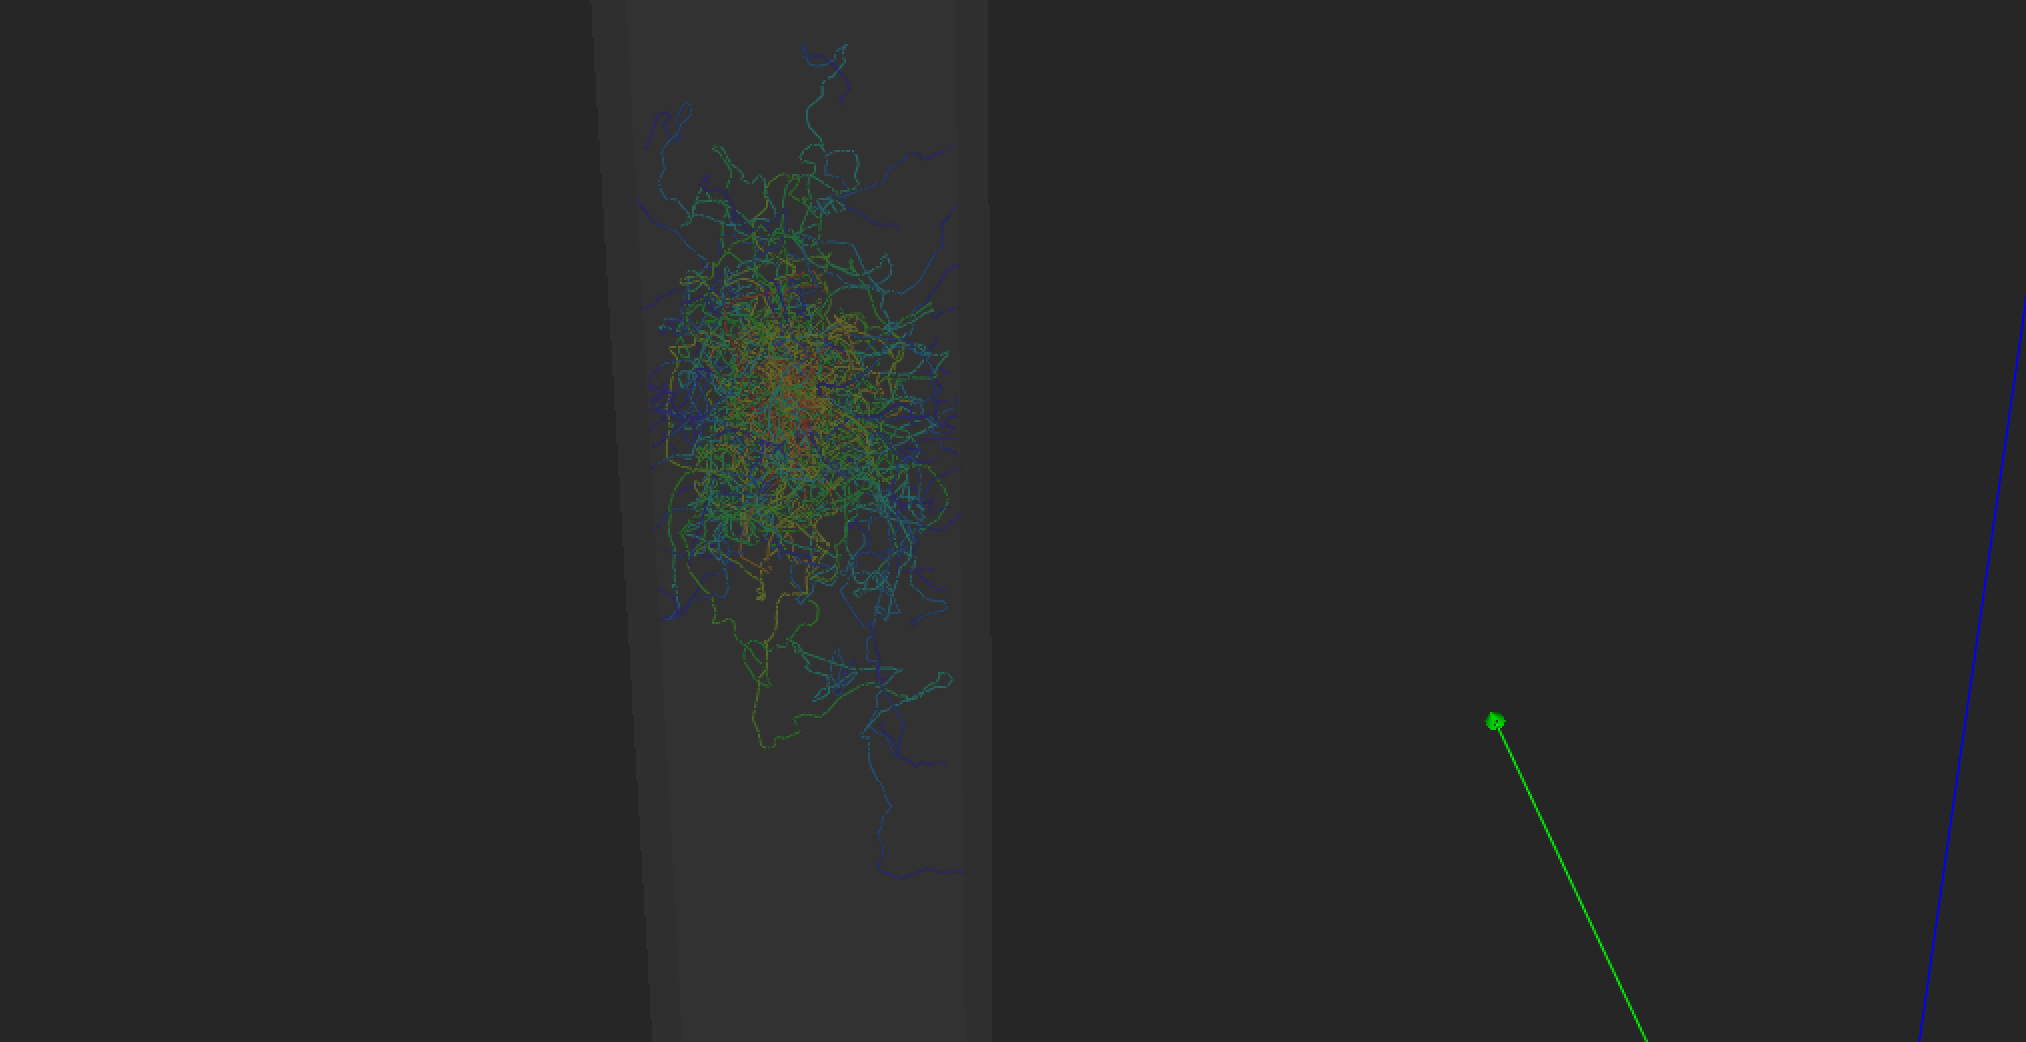
\includegraphics[width=\textwidth, trim={6cm 4cm 13cm 1.5cm}, clip]{img/instant-absorption-steamshovel-sahmoo8O-3d}
    \caption{View from the side.}
  \end{subfigure}
  \begin{subfigure}{.32\linewidth}
    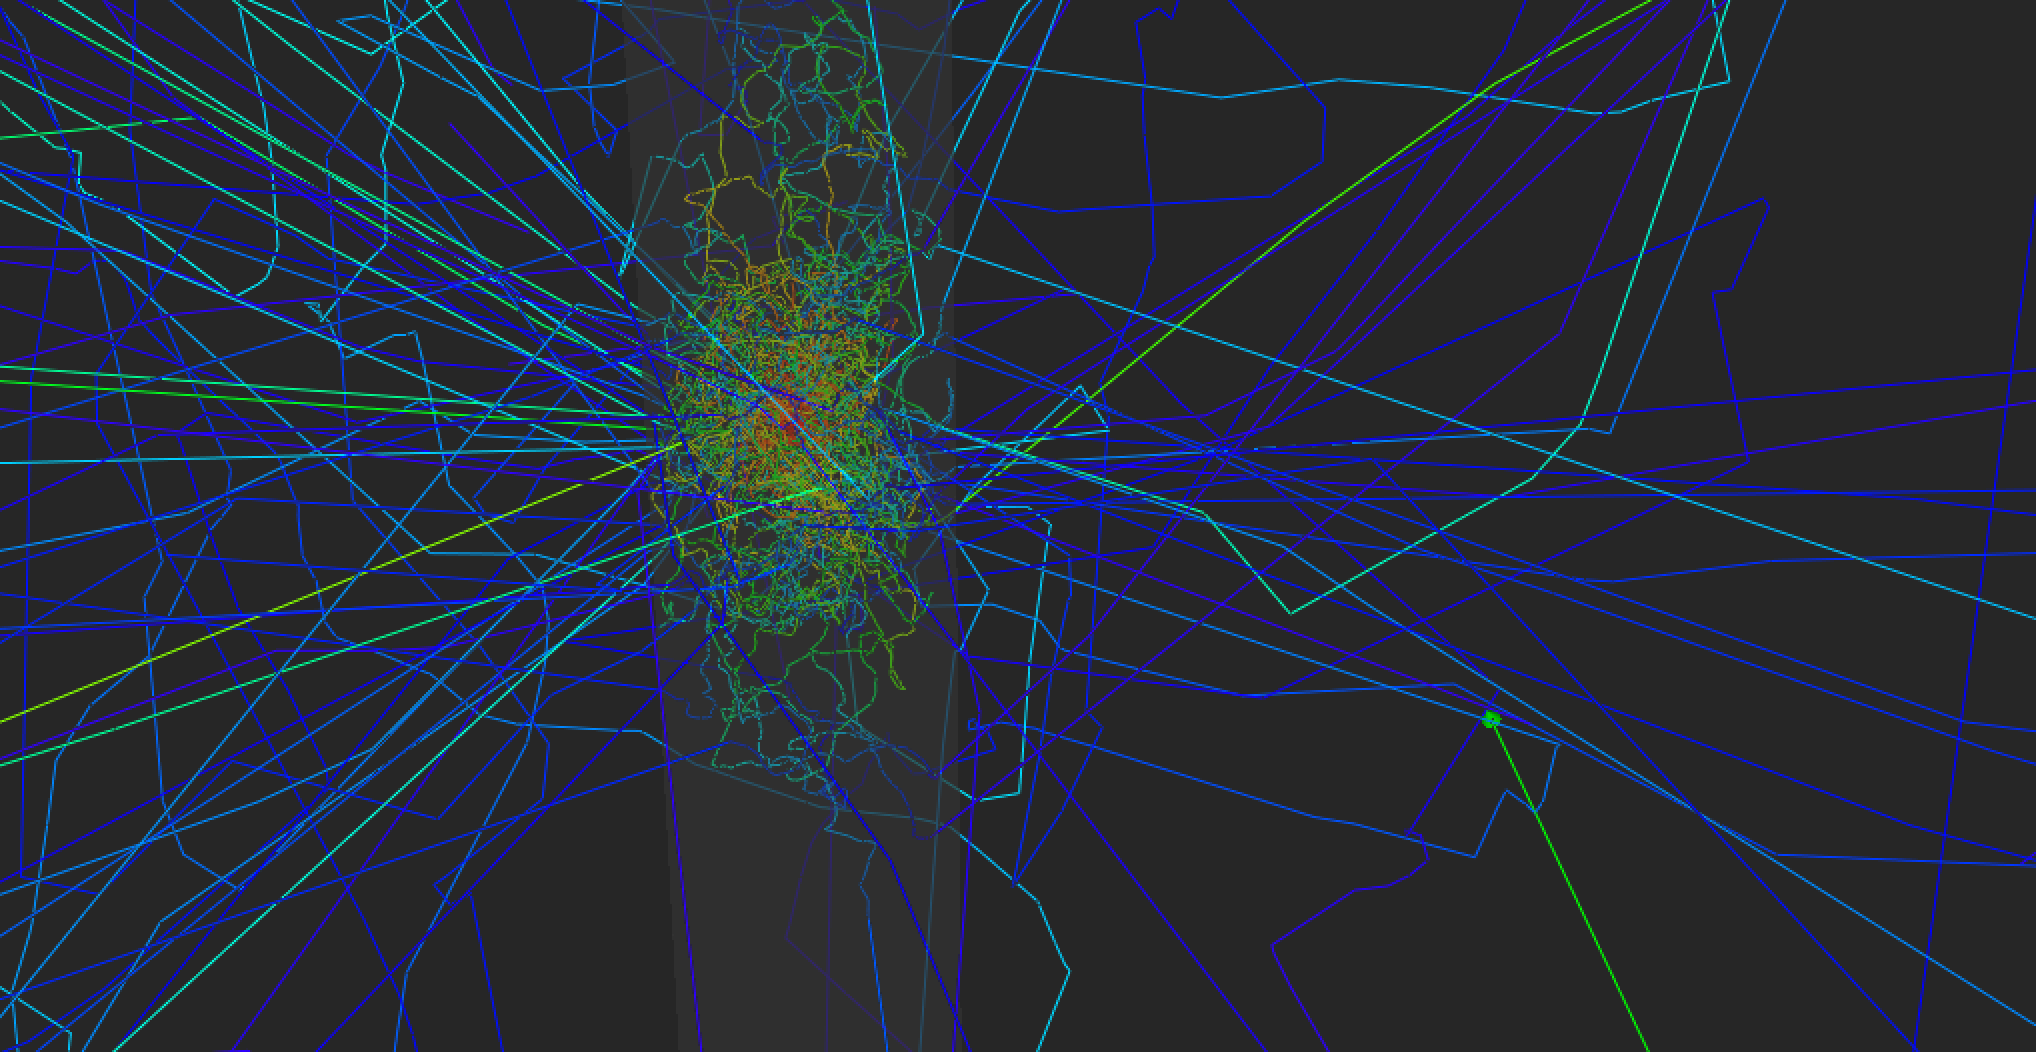
\includegraphics[width=\textwidth, trim={6cm 4cm 13cm 1.5cm}, clip]{img/instant-absorption-steamshovel-sahmoo8O-turned-off}
    \caption{Instant absorption turned off.}
  \end{subfigure}
  \caption{Visualizing an instant-absorption test where photons are started within two nested cylinders. The outer cylinder is configured for instant absorption. No photon can pass through the area between both cylinders unless the instant absorption is turned off.}
  \label{fig:sahmoo8O}
\end{figure}

### Absorption Length Distributions

- cross checks #63
- exponentieller abfall
  - without border #64
  - with 1 border #65
  - with 2 borders #66
- zylinder-übergang #47
- distance to hole-ice center #67
- distance to next scattering point #71
- scattering and absorption #72 (?)

